% -*- TeX-master: "../paper_notes.tex" -*-
\newpage
\section{Fabricating xMon \cite{Barends_2013}}
\label{sec:making-transmon}

\begin{framed}\noindent
  \red{\textbf{The original paper on the xMon}}\ec
  
  xMon is fabricated by  taking an Al covered wafer and etching out  narrow channels to define
  the qubit  and waveguides.   \red{\textbf{New type of  capacitance of the  xMon. New  way of
      passing transmission line in channel between ground planes.}}\ec

  \begin{center}
    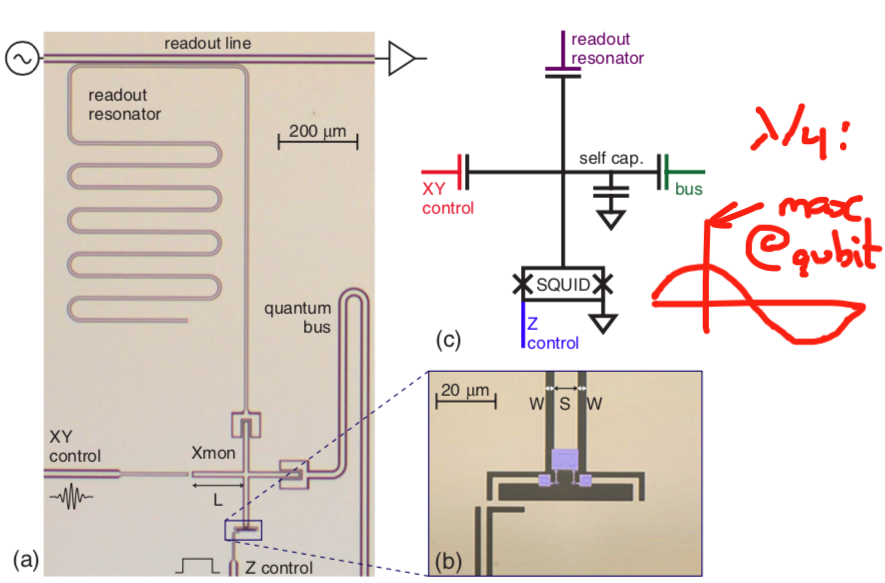
\includegraphics[height=9cm]{images/mxon/xmon_1}
  \end{center}

  \begin{itemize}
  \item $\frac{1}{2\pi}\omega_{21}$ = \iunit{6}{GHz}, $ E_{C}/E_J \approx 95 $
  \item Shape of the cross and connected to JJs at the bottom end (see the image);
  \item  Equivalent  to   the  transmon  \red{but  with  cross  in   place  of  interdigitated
      capacitance}\ec
    \begin{center}
      \includegraphics[height=4cm]{images/mxon/xmon_2}
    \end{center}
    \noindent
  \item Coherence time of 40\,$\mu$s;
  \item Very long times T$_1$=44$\mu$s and  T$_2$=20$\mu$s. The limit T$_2$=$\frac{1}{2}$ T$_1$ is
    not reached,  meaning that there  is additional T$_{\varphi}$. Do  by exciting state  and taking
    reading in the graph below.

  \begin{center}
    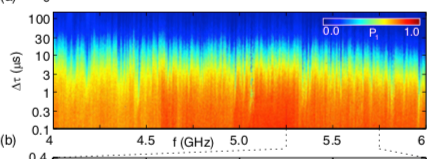
\includegraphics[height=4cm]{images/mxon/xmon_3}
  \end{center}

  \noindent
\end{itemize}

\subsection{Fabrication parameters}\label{sec:fabr-param}
\begin{enumerate}
\item \red{JJ size of 0.30$\times 0.20\,\mu$m$^2$}\ec;
\item \red{Tie the ground planes together at the capacitances}\ec;
\item Size of the cross:
  \begin{equation}
    \label{eq:images/mxon/xmon_cross}
    \begin{aligned}
      130 \le & \iunit{L\,\mu}{m} \le 170 \\
      8 \le & \iunit{W\,\mu}{m} \le 24 \\
      8 \le & \iunit{S\,\mu}{m} \le 24 \\
      second-line
    \end{aligned}
  \end{equation}
  
  \begin{center}
    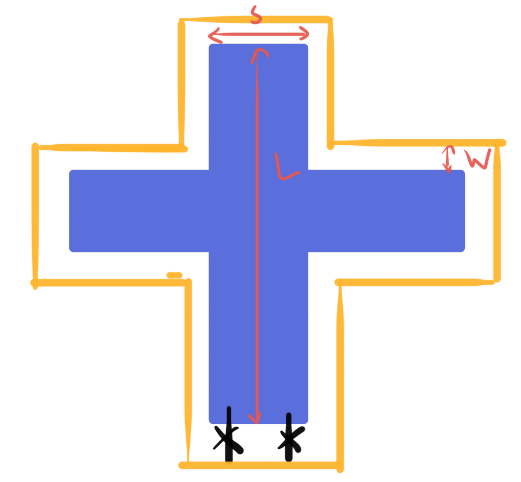
\includegraphics[height=5cm]{images/mxon/xmon_4}
  \end{center}

\item T$_1$  increases with  widths $  S $  and $ W  $.  (Widening  capacitor spreads  out the
  electric  field  distribution,  and  hence  lowers the  'surface  participation',  which  is
  essentially electric field density)
\end{enumerate}



  
\end{framed}
